\documentclass[landscape,twocolumn,a4paper]{article}
\setlength{\oddsidemargin}{-.6in}	 % default=0in
\setlength{\textwidth}{11in}	 % default=9in
\setlength{\columnsep}{0.5in}	 % default=10pt
\setlength{\columnseprule}{1pt}	 % default=0pt (no line)
\setlength{\textheight}{7.5in}	 % default=5.15in
\setlength{\topmargin}{-1.0in}	 % default=0.20in
\setlength{\headsep}{0.25in}	 % default=0.35in
\setlength{\parskip}{1.2ex}
\setlength{\parindent}{0mm}
\usepackage{titlesec}
\titlespacing*{\section}{0pt}{5pt}{-5pt}
\titlespacing*{\subsection}{0pt}{0pt}{-5pt}
\titlespacing*{\subsubsection}{0pt}{0pt}{-5pt}


%Math
\usepackage{amsmath}
\usepackage{amsfonts}
\usepackage{amssymb}
\usepackage{amsthm}
\usepackage{ulem}
\usepackage{stmaryrd} %f\UTF{00FC}r Blitz!
\usepackage{tikz}

\usepackage{multirow}
\usepackage{multicol}


%PageStyle
\usepackage[ngerman]{babel} % deutsche Silbentrennung
\usepackage[utf8]{inputenc} 
\usepackage{fancyhdr, graphicx}
\usepackage[scaled=0.92]{helvet}
%\usepackage{enumitem}
\usepackage{parskip}
%\usepackage[a4paper,top=2cm]{geometry}
%\setlength{\textwidth}{17cm}
%\setlength{\oddsidemargin}{-0.5cm}


%My Commands
\newcommand{\RN}{\mathbb{R}} %Real Number
\newcommand{\NN}{\mathbb{N}} %Natural Number
\newcommand{\QN}{\mathbb{Q}} %Rational Number
\newcommand{\ZN}{\mathbb{Z}} %ganze Zahlen
\newcommand{\CN}{\mathbb{C}}
\newcommand{\Teilt}{\mid} %|
\newcommand{\Teiltn}{\nmid} %kein teiler
\newcommand{\Potp}{\mathcal{P}} %Potenzmenge
\newcommand{\Pota}{\mathcal{A}}
\newcommand{\Potr}{\mathcal{R}}
\newcommand{\Potn}{\mathcal{N}}
\newcommand{\Bold}[1]{\textbf{#1}} %Boldface
\newcommand{\Kursiv}[1]{\textit{#1}} %Italic
\newcommand{\T}[1]{\text{#1}} %Textmode
\newcommand{\Nicht}[1]{\T{\sout{$ #1 $}}} %Streicht Shit durch
\newcommand{\lra}{\leftrightarrow} %Arrows
\newcommand{\ra}{\rightarrow}
\newcommand{\la}{\leftarrow}
\newcommand{\lral}{\longleftrightarrow}
\newcommand{\ral}{\longrightarrow}
\newcommand{\lal}{\longleftarrow}
\newcommand{\Lra}{\Leftrightarrow}
\newcommand{\Ra}{\Rightarrow}
\newcommand{\La}{\Leftarrow}
\newcommand{\Lral}{\Longleftrightarrow}
\newcommand{\Ral}{\Longrightarrow}
\newcommand{\Lal}{\Longleftarrow}
\newcommand{\Vektor}[1]{\vec{#1}}
\newcommand{\Brace}[1]{\left( #1 \right)} %()
\newcommand{\Bracel}[1]{\left\lbrace #1 \right.} %(
\newcommand{\Bracer}[1]{\right. #1 \right\rbrace} %)
\newcommand{\Brack}[1]{\left\lbrace #1 \right\rbrace} %{}
\newcommand{\Brackl}[1]{\left\lbrace #1 \right.} %{
\newcommand{\Brackr}[1]{\right. #1 \right\rbrace} %}
\newcommand{\Result}[1]{\underline{\underline{#1}}} %Doppelt unterstrichen
\newcommand{\Abs}[1]{\left| #1 \right|} %Absolutbetrag
\newcommand{\Norm}[1]{\Abs{\Abs{ #1 }}} %Norm
\newcommand{\Arrays}[1]{\left(\begin{array}{c}#1\end{array}\right)} %Array mit einer Kolonne ()
\newcommand{\Array}[2]{\left(\begin{array}{#1}#2\end{array}\right)} %Array mit n Kolonnen ()
\newcommand{\Bracka}[2]{\left\lbrace\begin{array}{#1}#2\end{array}\right\rbrace} %Array mit {}
\newcommand{\Brackal}[2]{\left\lbrace\begin{array}{#1} #2 \end{array}\right.} %Array mit {
\newcommand{\Brackar}[2]{\left.\begin{array}{#1} #2 \end{array}\right\rbrace} %Array mit }
\newcommand{\Sumone}[2]{\sum_{#2=1}^{#1}} %Summe von 1
\newcommand{\Sumz}[2]{\sum_{#2=0}^{#1}} %Summe von 0
\newcommand{\Sum}[2]{\sum_{#2}^{#1}} %Allgemeine Summe
\newcommand{\Oneover}[1]{\frac{1}{#1}} %1 über igendwas
\newcommand{\Tablewt}[3]{\begin{table*}[h]\caption{#1} \begin{tabular}{#2}{#3}\end{tabular}\end{table*}} %Table mit Titel
\newcommand{\Oben}[2]{\overset{#1}{#2}} %etwas über etwas anderem
\newcommand{\Unten}[2]{\underset{#1}{#2}} %etwas unter etwas anderem
\newcommand{\Bildcap}[2]{\begin{figure}[htb]\centering\includegraphics[width=0.2\textwidth]{#1} \caption{#2}\end{figure}} %Bild mit beschriftung
\newcommand{\Bildjpeg}[1]{\includegraphics[width=0.2\textwidth]{#1.jpeg}} %Bilder jpeg!!
\newcommand{\Bildjpg}[1]{\includegraphics[width=0.2\textwidth]{#1.jpg}} %Bilder jpg!!
\newcommand{\Bild}[1]{\includegraphics[width=0.4\textwidth]{#1}} %Bilder jpg!!
%Beispiel für lstlisting \lstinputlisting[label=Aufgabe 4a,caption=Aufgabe 4a]{4a.java}

% Code listenings
\usepackage{color}
\usepackage{xcolor}
\usepackage{listings}
\usepackage{caption}
\DeclareCaptionFont{white}{\color{white}}
\DeclareCaptionFormat{listing}{\colorbox{gray}{\parbox{\textwidth}{#1#2#3}}}
\captionsetup[lstlisting]{format=listing,labelfont=white,textfont=white}
\lstdefinestyle{JavaStyle}{
 language=Java,
 basicstyle=\footnotesize\ttfamily, % Standardschrift
 numbers=left,   % Ort der Zeilennummern
 numberstyle=\tiny,          % Stil der Zeilennummern
 stepnumber=5,              % Abstand zwischen den Zeilennummern
 numbersep=5pt,              % Abstand der Nummern zum Text
 tabsize=2,                  % Groesse von Tabs
 extendedchars=true,         %
 breaklines=true,            % Zeilen werden Umgebrochen
 frame=b,         
 %commentstyle=\itshape\color{LightLime}, Was isch das? O_o
 %keywordstyle=\bfseries\color{DarkPurple}, und das O_o
 basicstyle=\footnotesize\ttfamily,
 stringstyle=\color[RGB]{42,0,255}\ttfamily, % Farbe der String
 keywordstyle=\color[RGB]{127,0,85}\ttfamily, % Farbe der Keywords
 commentstyle=\color[RGB]{63,127,95}\ttfamily, % Farbe des Kommentars
 showspaces=false,           % Leerzeichen anzeigen ?
 showtabs=false,             % Tabs anzeigen ?
 xleftmargin=17pt,
 framexleftmargin=17pt,
 framexrightmargin=5pt,
 framexbottommargin=4pt,
 showstringspaces=false      % Leerzeichen in Strings anzeigen ?        
}

%Config
\renewcommand{\headrulewidth}{0pt}
\setlength{\headheight}{15.2pt}
\titleformat{\section}{\normalsize\bfseries}{\thesection}{1em}{}
\titleformat{\subsection}{\normalsize\bfseries}{\thesubsection}{1em}{}
\titleformat{\subsubsection}{\normalsize\bfseries}{\thesubsubsection}{1em}{}
\setlength{\parskip}{5pt}

%Metadata
\title{
	\vspace{5cm}
	Datennetze 2
}
\author{Manuel Jenny}
\date{4. Semester (FS 2013)}


% hier beginnt das Dokument
\begin{document}
\begin{footnotesize}
\section{VLAN Trunking Protocol VTP}

\subsection{Nutzen \& Begriffe}
\begin{itemize}
	\item Zentralisierung des VLAN Management
	\item Schnelles Einfügen eines zusätzlichen VLANs
	\item Konsistenz über ganzes Netz
	\item VTP-Domain: Gruppe von Switches, die VTP untereinander ausführen\\ $S(config)\#vtp$ $domain$ $DOMAIN_NAME$.
	\item VTP Advertisments: VTP-Infos werden über trunk Ports verteilt (Layer-2)
	\item VTP Modi (def. server): $S(config)\#vtp$ $mode$ $[server$ $|$ $client$ $|$ $transparent]$
	\item VTP Pruning: sorgt dafür, dass Advertisments nicht auf jedes IF geflutet werden.
\end{itemize}

\subsection{VTP Funktionen}
Praxis: Erst alle Switches konfigurieren, die \underline{NICHT} VTP-Server sein sollen\\

\subsubsection{VTP Domain}
\begin{itemize}
	\item Verteilung durch Server
	\item \underline{Achtung:} Verteilte Namen können nicht mehr einfach so überschrieben werden!
	\item Vorsicht beim Einbau eines neuen Switches (Verbreitung von falschen Infos)
\end{itemize}

\subsubsection{VTP advertisments}
%\includegraphics[scale=0.5]{vtp-ieee-header.png}\\
3 Arten von Advertisments:
\begin{itemize}
	\item Summary Advertisments: alle 5 Minuten mit aktueller Config
	\item Subset Advertisments: Änderungen von VLANs werden bekannt gegeben
	\item Request Advertisments: Client an Server, danach Summary Advertisment
\end{itemize}

\subsubsection{VTP Konfiguration}
\begin{tabular}{l | l}
	\textbf{Server} & \textbf{Client} \\
	\hline \\
	$S\#sh$ $vtp$ $status$ & $S\#sh$ $vtp$ $status$ \\
	$S(config)\#vtp$ $domain$ $myName$ & $S(config)\#vtp$ $mode$ $client$ \\
	$S(config)\#vtp$ $version$ $2$ & $S(config)\#vtp$ $version$ $2$ \\
	 & $S(config)\#vtp$ $password$ $myPW$
\end{tabular}


\section{Spanning Tree Protocol STP}
\subsection{Der ST Algorithmus}
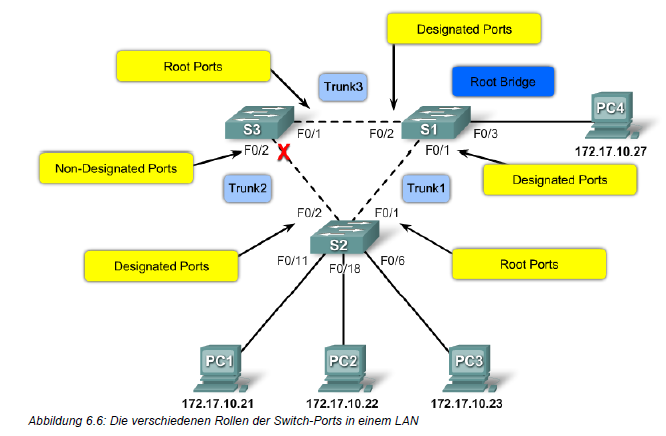
\includegraphics[scale=0.40]{stp.png}\\\\\\
\textbf{Ablauf:}
\begin{itemize}
	\item[1.)] Bestimmung Root Bridge (RB) (tiefste Bridge ID [Standard: MAC Adresse]).
	\item[2.)] Bestimmung der "root ports" (kürzester Weg zur Root Bridge [Link Metrik]).
	\item[3.)] Auf jedem LAN-Segment: Bestimmung des "designated ports".
	\item[4.)] "non-designated ports" (weder root noch designated ports) werden blockiert.
\end{itemize}

\subsection{Bridge ID}
\begin{itemize}
	\item Bridge Priority (2 Bytes) + MAC Address (6 Bytes)
	\item Bridge Priority (4 Bits) + Extended System ID (12 bits) + MAC Address (48 Bits)
	\item Bridge Priority: Kann nur in Schritten von 4096 verändert werden
	\item Extended System ID: gibt an, zu welchem VLAN der Rahmen gehört
	\item Somit hat ein Switch so viele Bridge IDs wie VLANs
\end{itemize}

\subsection{Port-Rollen \& STP Zustände}
\begin{itemize}
	\item Ermittlung des Root Ports (nächster zur Root Bridge [Link-Kosten])\\
	Kosten manipulieren: $S(config$--$if)\#spanning$--$tree$ $cost$ $25$
	\item Ermittlung des Designated Ports ("nächster" Port zur Root) | Falls $"$unentschieden":
	\begin{itemize}
		\item tiefere BID
		\item tiefere Port ID
	\end{itemize}
	\item Beeinflussbar durch höhere Priority:\\
	$S(config$--$if)\#spanning$--$tree$ $port$--$priority$ $112$
	\item Zustände: Disabled$\ra$Blocking$\ra$Listening$\ra$Learning$\ra$Forwarding
	\item Nachrichten: Topology Change Notification (TCN), Topology Change Acknowledgement (TCA), Topology Change (TC)
	\item Topologieänderung: Switch [TCN]$\ra$ RB | RB [TCA]$\ra$Switch | RB [TC]$\ra$All Switches
	\item Zustandsänderung: [TCN]$\ra$Blocking$\ra$Listening$\ra$Learning$\ra$Forwarding
\end{itemize}

\section{Point-to-Point Protocol PPP}
\subsection{Serielle Punkt-zu-Punkt Verbindungen}
\begin{itemize}
	\item Einsatz: Layer-2-Protocol eingesetzt, um zwei Knoten miteinander zu verbinden
	\item über möglichst alle Medien laufen (Kupferkabel, Glasfaser, etc.)
	\item Unterstützung verschiedener gleichzeitig laufender Layer-3-Protokolle
	\item Data Terminating Equipment (DTE): LAN-Abschlussgerät (z.B. Router)
	\item Data Communication Equipment (DCE): WAN-Abschlussgerät (Telecom $\ra$ NTU $\ra$ definiert Takt)
	\item High Level Data Link Control (HDLC): PPP baut auf HDLC auf
	\item HDLC: Receive + Send Sequence Number $\ra$ kann fehlerhafte Rahmen wiederholen lassen
	\item HDLC-Konfiguration: $R(config-if)\#encapsulation$ $hdlc$
\end{itemize}

\subsection{Konzepte \& Konfiguration von PPP}
\subsubsection{PPP enthält 3 Unterprotokolle:}
\begin{itemize}
	\item Rahmenbildung (ähnlich wie HDLC)
	\item Link Control Protocol (LCP): Hinauffahren, Konfiguration und Test des Links
	\item Network Control Protocol (NCP): Um versch. Layer-3-Protokolle zu konfigurieren
\end{itemize}

\subsubsection{Aufbau einer PPP Verbindung}
\begin{itemize}
	\item[1.] Phase: Link Establishment, Aushandlung von Optionen
	\item[2.] Phase (optional): Kontrolle der Linkqualität (Fehlerrate)
	\item[3.] Phase: Aushandlung der Layer-3-Optionen
\end{itemize}

\subsubsection{PPP Konfiguration}
$R(config$--$if)\#encapsulation$ $ppp$\\
$R(config$--$if)\#compress$ $[stack$ $|$ $predictor]$\\
$R(config$--$if)\#ppp$ $quality$ $80$\\
$R(config$--$if)\#ppp$ $multilink$

\subsubsection{PPP Authentication}
Password Authentication Protocol (PAP) und Challenge Handshake Authentication Protocol (CHAP) (PAP \underline{NICHT} mehr sicher, da Passwort Klartext gesendet wird)\\
$R1(config)\#username$ $R3$ $password$ $cisco$\\
$R(config$--$if)\#ppp$ $authentication$ $chap$


\section{Frame Relay}
FR erledigt:
\begin{itemize}
	\item Rahmenbildung
	\item Zugang zum Netz
	\item "switcht" Rahmen ans Ziel
	\item gibt Rahmen in richtiger Reihenfolge ab
	\item Fehler werden erkannt, aber nicht korrigiert
\end{itemize}
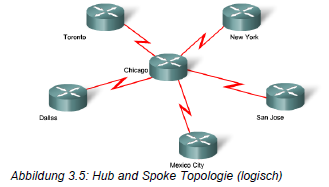
\includegraphics[scale=0.3]{hub-spoke-logisch.png}
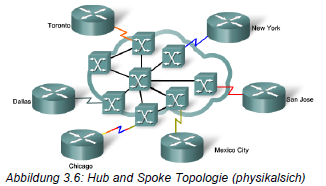
\includegraphics[scale=0.3]{hub-spoke-physikalisch.png}
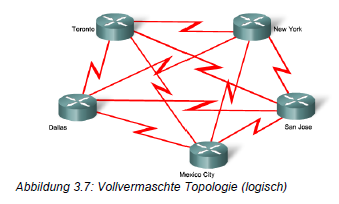
\includegraphics[scale=0.3]{vollvermascht-logisch.png}
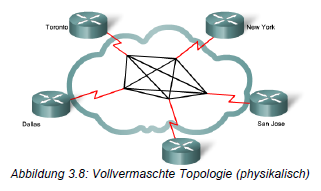
\includegraphics[scale=0.3]{vollvermascht-physikalisch.png}\\
\subsection{Zuordnung FR VC zu IP}
Local Management Interface LMI umfasst:
\begin{itemize}
	\item Virtual Circuit (VC) status message: sollte VC gelöscht werden wird Frame Relay Access Device (FRAD), welches beim Kunden steht, informiert.
	\item Multicasting: Rahmen wird an eine Gruppe von Zielen gesendet
	\item Global Addressing: Gibt Data Link Connection Identifiers (DLCIs) [da FR verbindungsorientiert ist], die globale Bedeutung haben
	\item Simple flow control: Xon/Xoff Mechanismus für Protokoll-Suiten ohne Flusskontrollen
\end{itemize}
\subsection{Konfiguration}
Inverses ARP ausschalten:\\
$R(config$--$if)\#encapsulation$ $frame$--$relay$ $ietf$\\
$R(config$--$if)\#no$ $frame$--$relay$ $inverse$--$arp$\\
Statisches Mapping:\\
$R(config$--$if)\#frame$--$relay$ $map$ $ip$ $XXX.XXX.XXX.XXX$ $102$ $broadcast$\\
$R(config$--$if)\#int$ $s0/0/1.112$ $point$--$to$--$point$\\
$R(config$--$subif)\#encapsulation$ $frame$--$relay$ $ietf$\\
$R(config$--$subif)\#ip$ $address$ $[IP]$ $[SUBNET]$\\
$R(config$--$subif)\#frame$--$relay$ $interface$--$dlci$ $115$


\section{Access Control Lists ACLs}
TBD!!!
\newpage
\section{IP Adressierungsdienste (DHCP, NAT, IPv6)}
\subsection{DHCP}
\subsubsection{Einführung}
Folgendes wird für Kommunikation benötigt:
\begin{itemize}
	\item MAC-Adresse (Schicht 2)
	\item eine Schicht-3-Adresse
	\item eine Subnetz-Maske
	\item ein Default Gateway und
	\item die Adresse eines DNS Servers
\end{itemize}
DHCP Server hat Aufgabe, Arbeitsstationen beim Aufstarten mit nötigen Parametern zu versorgen. Er verwaltet die IP-Adressen.
\subsubsection{Funktion von DHCP}
Drei verschiedene Mechanismen:
\begin{itemize}
	\item Manuelle Vergabe: Admin vergibt Host gezielt IP-Adresse, DHCP teilt Adresse dem Client mit.
	\item Automatische Vergabe: DHCP vergibt Host statische IP aus Pool. Es wird keine Lease-Time vereinbart! $\ra$ permanente Vergabe
	\item Dynamische Vergabe: DHCP vergibt IPs aus Pool dynamisch. Lease-Time wird von DHCP-Server bestimmt. Wird IP nicht mehr gebraucht, teilt dies der Client am Server mit.
\end{itemize}
Ablauf der dynamischen Vergabe:\\
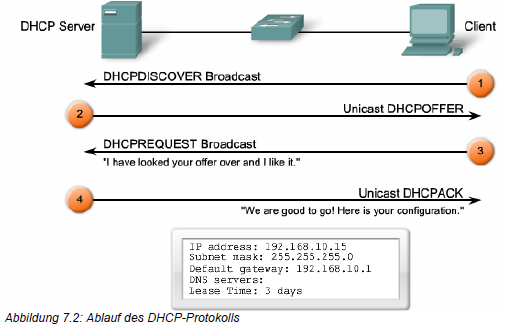
\includegraphics[scale=0.5]{ablauf-dhcp-protokoll.png}

\subsubsection{BOOTP \& DHCP}
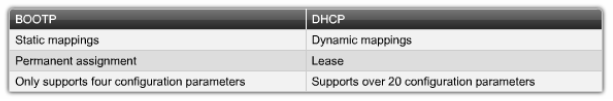
\includegraphics[scale=0.5]{bootp-dhcp.png}\\
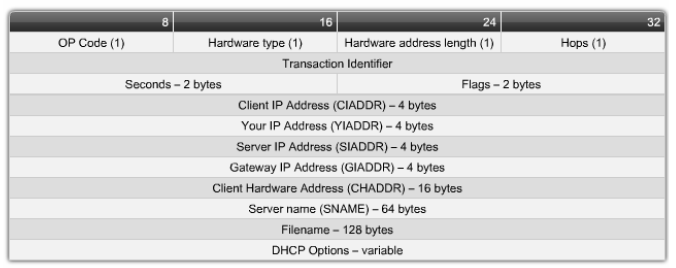
\includegraphics[scale=0.5]{dhcp-message-format.png}\\
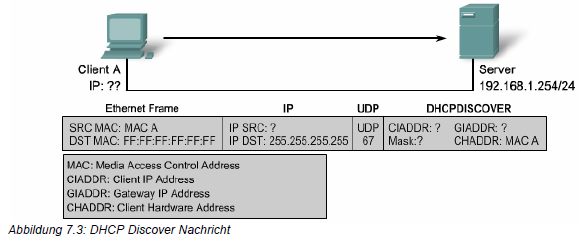
\includegraphics[scale=0.4]{dhcp-ablauf-1.png}
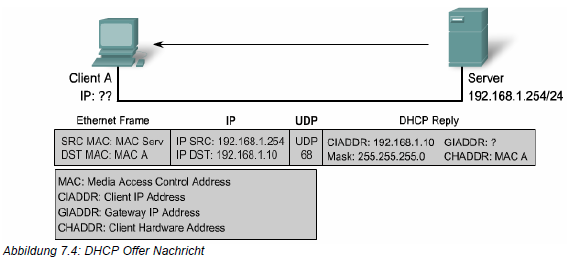
\includegraphics[scale=0.4]{dhcp-ablauf-2.png}\\
Danach folgt ein DHCP Acknowledge Paket.
\subsubsection{Konfiguration DHCP (1./2. = Server; 3. = Client)}
\begin{itemize}
	\item[1.)] Reserv. Adressbereich:
	$R1(config)\#ip$ $dhcp$ $exclude$--$address$ $[LOW ADDR]$ $[HIGH ADDR]$
	\item[2.)] Pool: $R1(config)\#ip$ $dhcp$ $pool$ $[POOLNAME]$\\
	$R1(config)\#network$ $[ADDR]$ $[MASK]$\\
	$R1(config)\#default$--$router$ $[ADDR]$\\
	$R1(config)\#dns$--$server$ $[ADDR]$\\
	$R1(config)\#domain$--$name$ $[NAME]$\\
	$R1(config)\#netbios$--$name$--$server$ $[ADDR]$
	\item[3.)] $S1(config$--$if)\#ip$ $address$ $dhcp$
\end{itemize}
\subsubsection{DHCP Relay}
Dient dazu Anfragen von zwei Netzen weiterzuleiten (Bsp. 192.168.10.X nach 192.168.11.5).\\
$R1(config)\#int$ $fa0/0$ $\Ra$ (192.168.10.X-Netz)\\
$R1(config$--$if)\#ip$ $helper$--$address$ $192.168.11.5$


\end{footnotesize}
\end{document} 